\documentclass[a4paper, 14pt]{report}
\usepackage[utf8]{inputenc}
\usepackage{graphicx}
\usepackage{subcaption}
\usepackage{float}
\usepackage{geometry}
 \geometry{
 a4paper,
 total={170mm,257mm},
 left=22mm,
 top=22mm,
 }

\title{Graph Report on Time taken in Parallel Computing\\CS251}
\author{Siddharth Chinmay\\160685}

\begin{document}

\maketitle

\chapter{Scatter plots}

\begin{figure}[H]
\centering
\includegraphics[width=1\textwidth]{scatter_1.eps}
 \caption{Scatter plot using 1 thread}
\end{figure}

\vskip 0.5in
{\Large As the number of elements increase, the time taken should increase, which is evident from the scatter plots. The scatter plots are concentrated in one place for single thread as we are performing the same action 100 times. 1 thread computing takes the most time.}


\begin{figure}[H]
\centering
\includegraphics[width=1\textwidth]{scatter_2.eps}
 \caption{Scatter plot using 2 threads}
 \label{fig:cc_get}
\end{figure}

\vskip 0.5in
{\Large As the number of elements increase, the time taken should increase, which is evident from the scatter plots. 2 thread computing takes lesser time than 1 thread.}

\begin{figure}[H]
\centering
\includegraphics[width=1\textwidth]{scatter_4.eps}
 \caption{Scatter plot using 4 threads}
\end{figure}

\vskip 0.5in
{\Large As the number of elements increase, the time taken should increase, which is evident from the scatter plots. 4 thread computing takes least time.}

\begin{figure}[H]
\centering
\includegraphics[width=1\textwidth]{scatter_8.eps}
 \caption{Scatter plot using 8 threads}
 \label{fig:cc_get}
\end{figure}

\vskip 0.5in
{\Large As the number of elements increase, the time taken should increase, which is evident from the scatter plots. 8 thread computing takes time more than 4 threads but less than 1 thread as there are only 4 cores.}

\begin{figure}[H]
\centering
\includegraphics[width=1\textwidth]{scatter_16.eps}
 \caption{Scatter plot using 16 threads}
\end{figure}

\vskip 0.5in
{\Large As the number of elements increase, the time taken should increase, which is evident from the scatter plots. 16 thread computing takes time approximately equal to 8 thread computing.}

\chapter{Line plot}

\begin{figure}[H]
\centering
\includegraphics[width=1\textwidth]{thread_compare.eps}
 \caption{Line plot showing average time taken using 1,2,4,8 or 16 threads}
\end{figure}

\vskip 0.5in
{\Large As the processor if 4 core processor, time taken is minimum for 4 threads. It is maximum for 1 thread which is equivalent to sequential processing. Also, lineplots for 8 and 16 threads are approximately equal because they process in a same way.}

\chapter{Bar Graphs}

\begin{figure}[H]
\centering
\includegraphics[width=1\textwidth]{speedup.eps}
 \caption{Bar Graph showing Speedup vs Number of elements in various threads}
\end{figure}

\vskip 0.5in
{\Large Less number of elements don't show much difference in speedup for parallel computing which we can clearly see in the bar graph. Speedup is maximum for 4 threads which reaches 3, so it is not ideal. An ideal parallel computing should have Speedup = Number of threads.}

\begin{figure}[H]
\centering
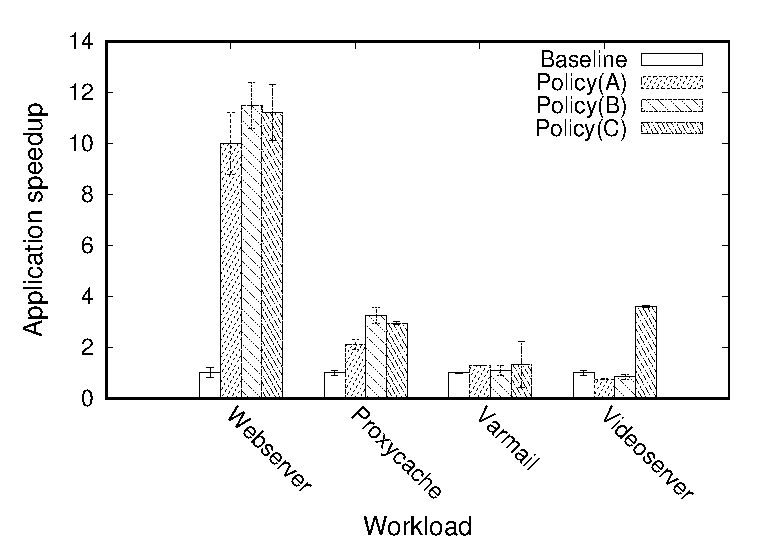
\includegraphics[width=1\textwidth]{speedup_errorbar.eps}
 \caption{Bar graph with error bars}
\end{figure}

\vskip 0.5in
\noindent
{\Large Errorbars show that the data for time taken recorded show large deviations from mean value and decreases for 2, 4 threads but increases for 8, 16 threads when compared to single thread computing.}

\end{document}